\chapter{Report and discussion of research results}

\section{Calibration hyper-parameters}

Picking the optimal bin size can be done via cross-validation. However, since we have a fairly large amount of data points, we simply set the bin size to be 1000 for POS tagging, 400 for Tweet POS tagging and 10000 for coreference resolution. 

We report the calibration score and its confidence intervals for all our experiments. To compute the score, we implement the method described in section 3.2.2 with a sample of size of 1000.

\section{Part-of-speech tagging}

\subsection{Data}

We extract WSJ articles from the CoNLL-2011 dataset for this experiment. The original data set has already been split the into training, development and testing sets so we filter WSJ articles from each set and join the sentences into together. This process results in 11772 sentences for training, 1632 sentences for development and 1382 sentences for testing. Running the models on the testing set produces 30543 prediction-observation pairs. We then conduct calibration analysis on this set of pairs. The query tested is whether a word has the ``NN'' tag. 

We train a HMM model using maximum likelihood principle. For CRF training, we implement the L2-regularized mini-batch AdaGrad method \citep{duchi2011adaptive}. The batch size is chosen via cross-validation.   

\subsection{Results}

\begin{figure}[t]
\begin{subfigure}{0.32\textwidth}
  \centering
  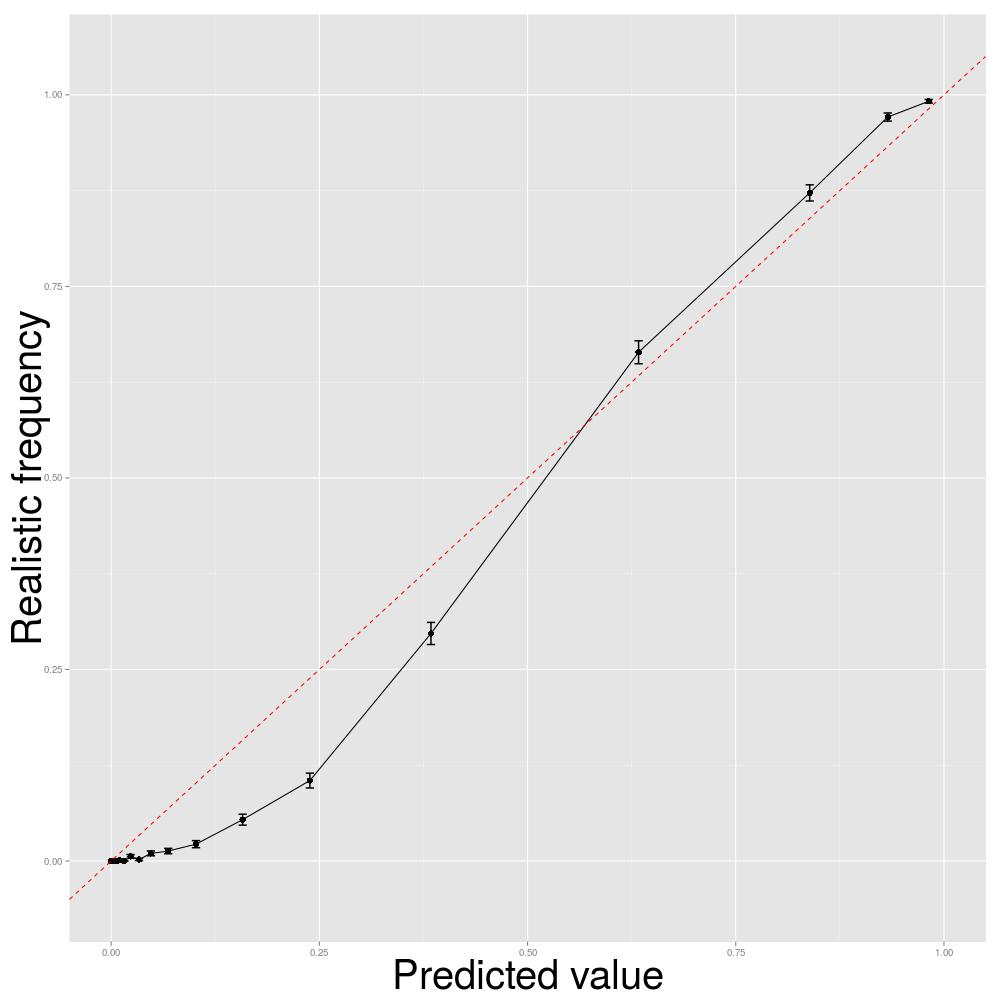
\includegraphics[width=\linewidth]{pos_hmm.jpg}
  \caption{}
\end{subfigure}
\begin{subfigure}{0.32\textwidth}
  \centering
  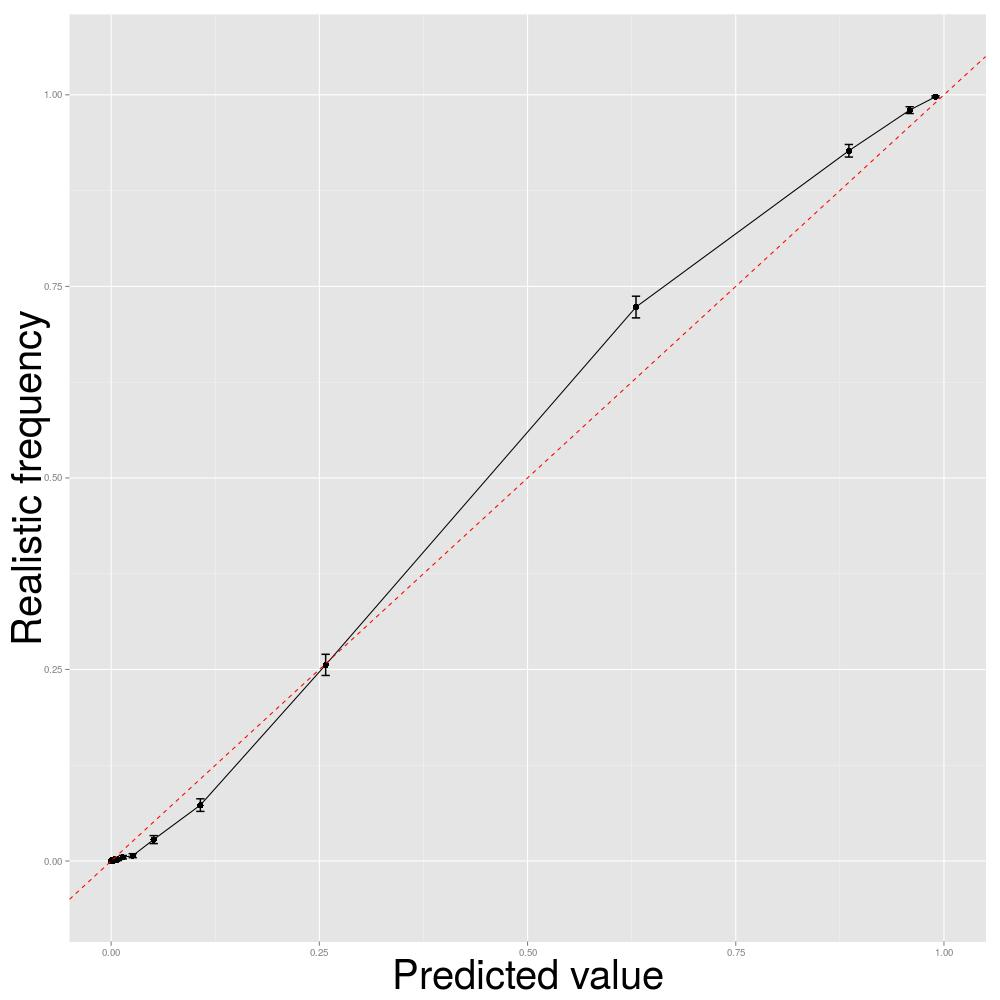
\includegraphics[width=\linewidth]{pos_crf.jpg}
  \caption{}
\end{subfigure}
\begin{subfigure}{0.32\textwidth}
  \centering
  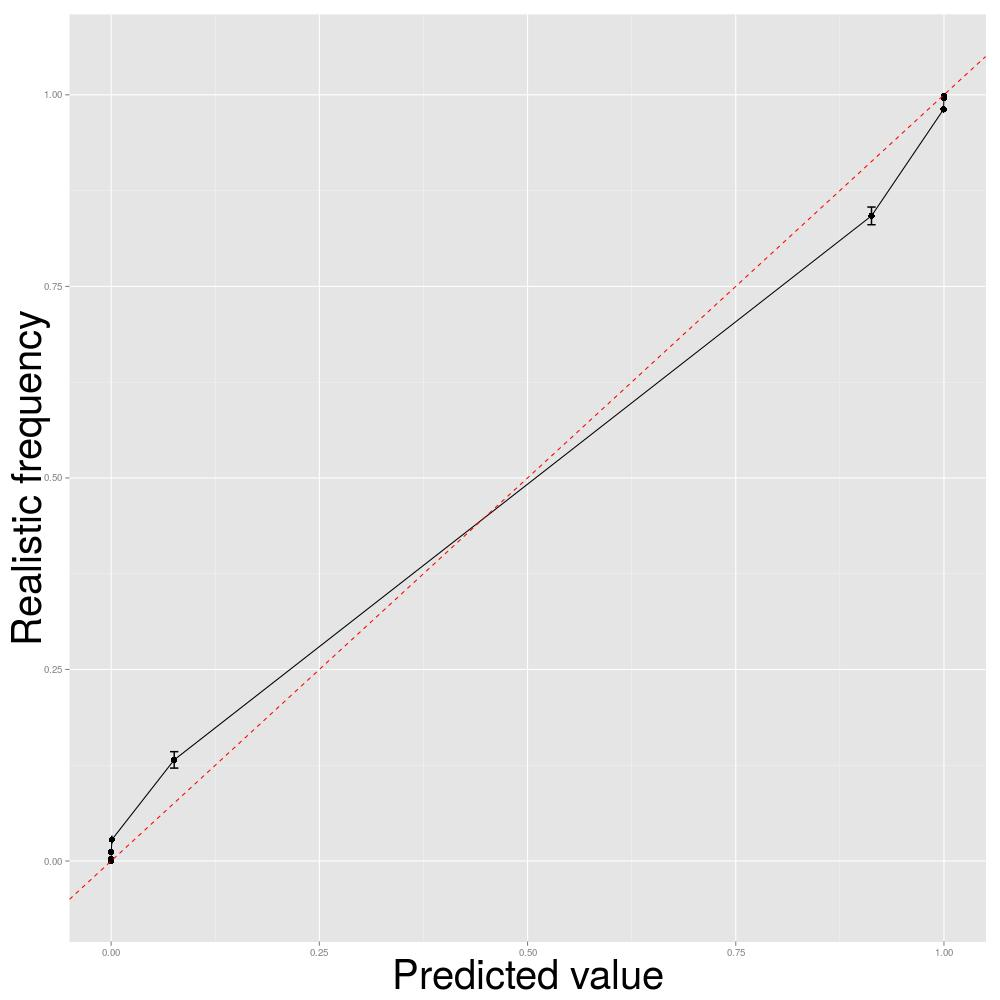
\includegraphics[width=\linewidth]{pos_crf_full.jpg}
  \caption{}
\end{subfigure}
\caption{Calibration curves for HMM and CRF models (POS tagging) (a) HMM (b) CRF with basic features (c) CRF with advanced features} 
\end{figure}

\begin{figure}[t]
  \centering
  \footnotesize
  \begin{tabular*}{0.57\textwidth}{@{\extracolsep{\fill}} | c | c | c | }
    \hline
    Model & Accuracy (\%) & CalibScore \\ 
    \hline
    HMM & 88.10 & 0.042 $\pm$ 5.27e-5 \\
    \hline
    CRF-Basic & 93.02 & 0.021 $\pm$ 6.81e-5 \\
    \hline
    CRF-Advanced & 96.08 & 0.018 $\pm$ 6.11e-5 \\
    \hline
  \end{tabular*}
\caption{Accuracy and calibration scores of the models for POS.}
\end{figure}

Firstly, we compare HMM with a CRF model with basic features (CRF-Basic). As mentioned in section 3.4.1, CRF-Basic contains only the transition features and the emission features. Figures 4.1(a) and 4.1(b) show calibration curves of the two models. CRF-Basic attains a significantly lower calibration score than HMM does (Figure 4.2). Moreover, the CRF-Basic's calibration has less mid-range points that of HMM, which indicates that the model generates more refined predictions.

To measure the affect of features on calibration, we add advanced features such as surrounding words, word shape, word length, prefixes and suffixes to CRF-Basic. We discover that as we use better features, we obtain more refined and calibrated predictions. The better featurized CRF (CRF-Advanced), which achieves a 96\% accuracy on the task, produces a calibration curve just slightly off the PCC (Figure 4.1(c)). 

\section{Twitter part-of-speech tagging}
\subsection{Data}

\begin{figure}[t]
\begin{subfigure}{0.32 \textwidth}
  \centering
  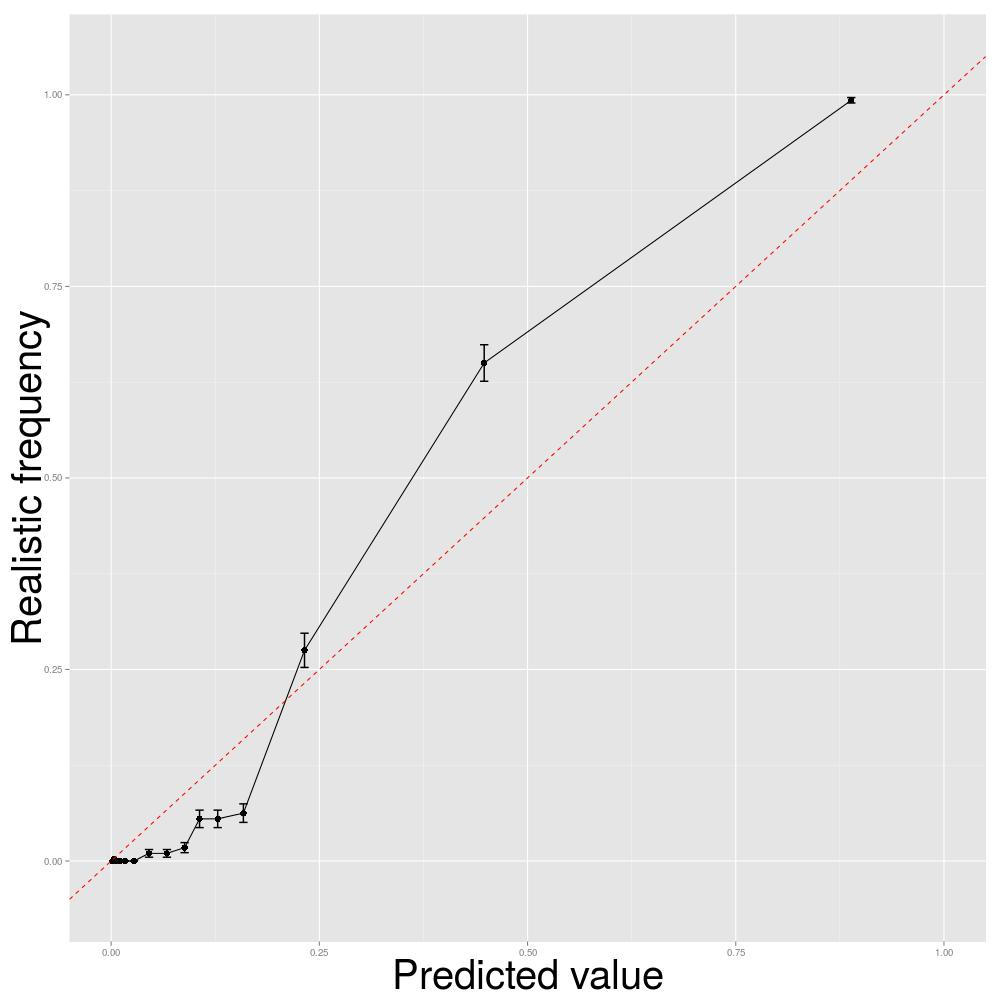
\includegraphics[width=\linewidth]{pos_tweet_hmm.jpg}
  \caption{}
 \end{subfigure}
\begin{subfigure}{0.32 \textwidth}
  \centering
  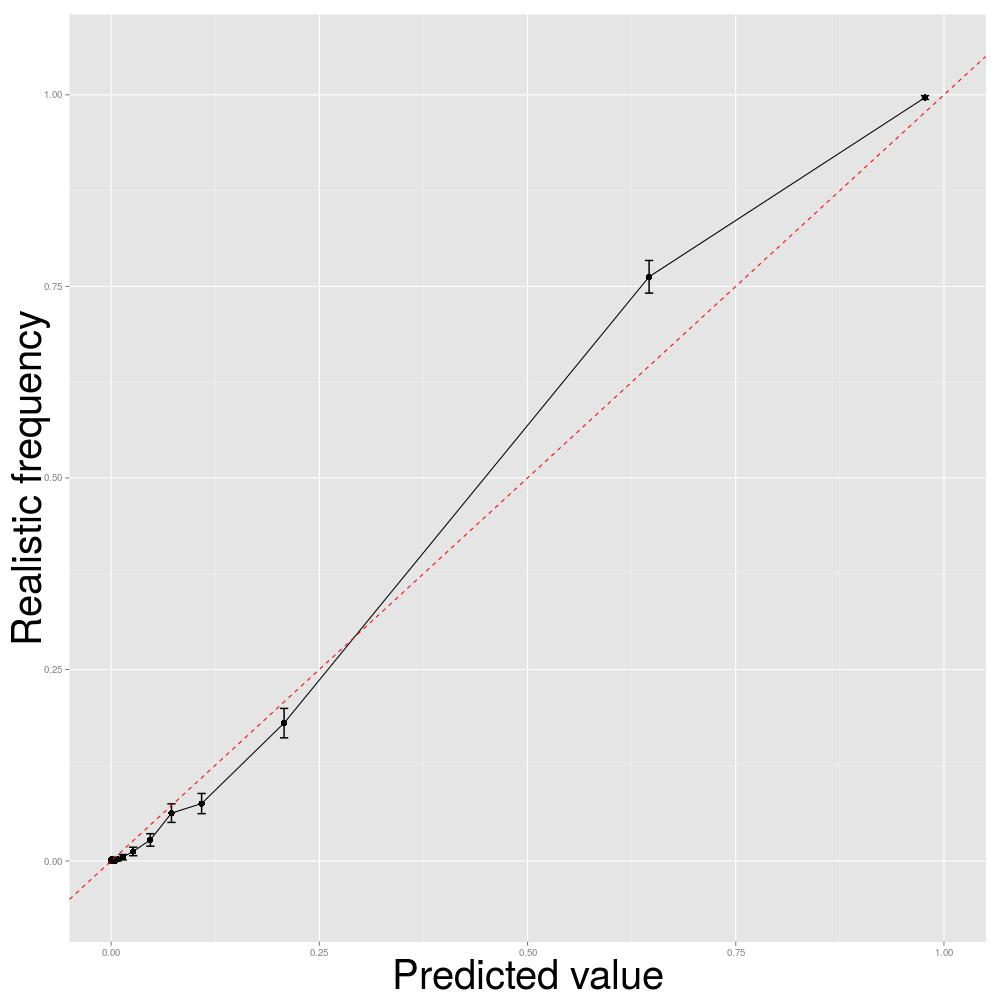
\includegraphics[width=\linewidth]{pos_tweet_crf.jpg}
  \caption{}
\end{subfigure}
\begin{subfigure}{0.32 \textwidth}
  \centering
  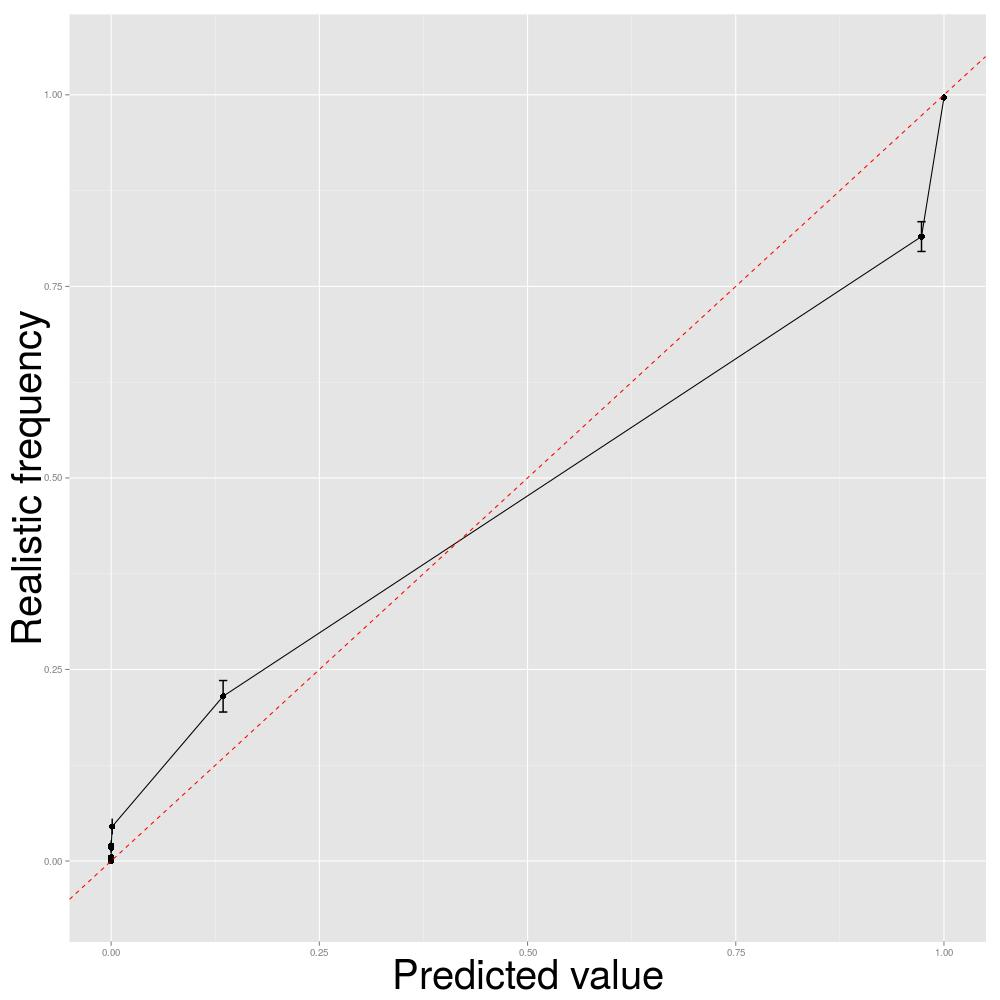
\includegraphics[width=\linewidth]{pos_tweet_crf_full.jpg}
  \caption{}
\end{subfigure}
\caption{Calibration curves for HMM and CRF models (TweetPOS) (a) HMM (b) CRF with basic features. (c) CRF with advanced features} 
\end{figure}

\begin{figure}[t]
  \centering
  \footnotesize
  \begin{tabular*}{0.57\textwidth}{@{\extracolsep{\fill}} | c | c | c | }
    \hline
    Model & Accuracy (\%) & CalibScore \\ 
    \hline
    HMM & 67.55 & 0.075 $\pm$ 1.40e-4 \\
    \hline
    CRF (Basic) & 78.12 & 0.034 $\pm$ 1.61e-4 \\
    \hline
    CRF (Advanced) & 86.19 & 0.048 $\pm$ 1.47e-4 \\
    \hline
  \end{tabular*}
\caption{Accuracy and calibration scores of the models for TweetPOS.}
\end{figure}


We repeat the same analysis in section 4.2 predicting POS tags for tweets. For this experiment, we use the ARK's Twitter POS data set \citep{gimpel2011part}, which consists of 1000 sentences for training, 327 sentences for development, 500 sentences for testing. The number of prediction-observation pairs obtain from testing set is 6160. Unlike the regular POS experiment, The query tested is whether a word has the ``V'' tag since we find that predicting ``N'' on tweets is still easy for the models.

\subsection{Results}

Comparing between HMM and CRF-Basic, we observe the same pattern as in the section 4.2. CRF-Basic gives a more calibrated and sharper predictions than HMM (Figure 4.3). In both experiments, the calibration score of HMM is always twice as large as that of CRF-Basic. On the other hand, unlike the previous experiment, adding more features to CRF worsens the calibration score (Figure 4.4). While CRF-Advanced produces sharper predictions, it is overconfident at high-score predictions. There are two possible explanations for this phenomenon. First, the data size is smaller; hence, the score may be not approximated well enough. Second, the feature set increases the recall but not the precision of the model.

\section{Coreference resolution}

\subsection{Data}

For this experiment, we use the available implementation of the Bekerley coreference resolution (Berkeley-coref) \citep{durrett2013easy}. The data set used is the CoNLL-2011 data set. The performance score of this system was around 62\% on the development set. The query tested is whether two mentions belong to the same entity. We apply calibration analysis on about 4 millions predictions generated from the development set. 

\subsection{Results}

\begin{figure}[t]
  \centering
  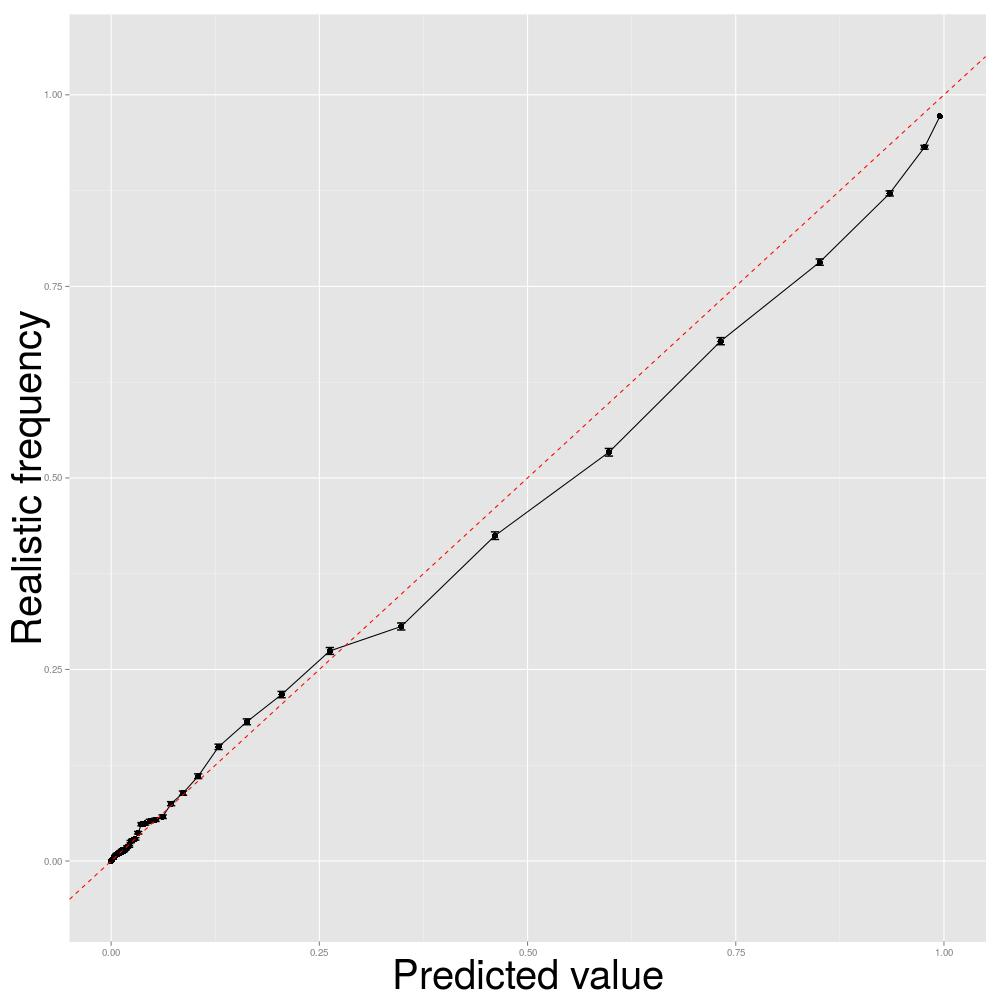
\includegraphics[width=0.5\linewidth]{coref.jpg}
  \caption{Calibration curve of Berkeley-coref.} 
\end{figure}

Although having a far-from-perfect accuracy score, the Berkeley's predictions are extremely reliable (Figure 4.5). Its calibration score is 0.007 $\pm$ 6.32e-6, much smaller than the models for the easier POS tagging task in the previous sections. The results also help explaining the effect of features on calibration. Berkeley-coref employs a carefully selected set of features called SURFACE. Whereas in the TweetPOS experiment, we see that adding features can degrade calibration, in this experiment, we observe a model with a good set of features can be very reliable despite making a lot of mistakes. The result of this experiment also confirms that discriminative models, with quality features, produces highly reliable predictions.    
